\documentclass[conference]{IEEEtran}
%\usepackage{draftwatermark}
\usepackage{graphicx}
\usepackage{cite}
\usepackage[belowskip=-10pt,aboveskip=2pt]{caption}
\usepackage[cmex10]{amsmath}
\usepackage{tikz}
\usepackage{csquotes}
\usetikzlibrary{patterns}
\usetikzlibrary{positioning}
\usetikzlibrary{arrows}
\usetikzlibrary{decorations.markings}
\newcommand{\todocomment}[2]{{\bf\sc (* from #1: #2 *) }}

\begin{document}

\title{Detecting Asteroids with Neural Networks}

\author{
\IEEEauthorblockN{Dustin~S.~Ingram}
\IEEEauthorblockA{Department of Computer Science\\
Drexel University, Philadelphia, PA\\
Email: dustin@cs.drexel.edu}
}

\maketitle

\begin{abstract}
In this project, I will use and compare various feature sets and methods for
building a neural network for use in detecting asteroids in astrophotography
data. I will propose three key features which can be used to train neural
networks to detect asteroids in this form of data: hue ratio, cluster
collinearity, and mean cluster distance, and prove their usefulness by
evaluating the accuracy of the resulting neural network. The results show that
neural networks are a fast and reliable form of classifiers for detecting
asteroids.
\end{abstract}

\section{Introduction}
The Sloan Digital Sky Survey~\cite{Gunn92thesloan} is ``one of the most
ambitious and influential surveys in the history of astronomy.'' It is
comprised of an open data set of images which together represent a scan of over
thirty-five percent of the observable sky, making it also the largest uniform
survey of the sky ever accomplished. The resulting data consists of hundreds of
thousands of images of various celestial bodies, but particularly interesting to
us is the millions of asteroids which exist in our solar system and,
potentially, cross Earth's orbit.

By exploiting a characteristic of the charge-coupled devices (CCDs) that the
Sloan Digital Sky Survey uses to collect it's image data, it is possible to
detect asteroids, their size and direction, amongst other properties. Because
the survey produces images in five different bands, any body moving across the
field of view of the instrument appears in different locations on each
individual exposure.

This problem is particularly good for neural networks, for a number of reasons.
First, we have a clear set of training data, and we are able to say with
confidence that any given training data point is valid ($1$) or invalid ($0$).
We are able to resolve each of the individual features to a $0 \to 1$ metric,
and there is a small amount of features (totaling three) which can accurately
define an item. Finally, using a neural network will create an extremely fast
and accurate classifier, which can be re-trained on the data is has classified
(after manual verification) to become even more accurate.

\section{Background}
There are a number of ways to perform asteroid detection on astrophotography
data, most of which are dependent on the characteristics and features of the
systems used to collect the data. For example, a well known but inefficient
approach to detecting any moving body in such data in such a situation, where
the moving object appears in different locations for different exposures, is to
remove all color from the images, greatly increase the contrast of both, invert
the images (so the background is white and the bodies are black) and rapidly and
successively blink the two images back and forth. Any moving body will
``toggle'' between it's two locations, and will therefore be somewhat apparent
to the naked eye.

A more efficient approach benefiting from this characteristic is that of
``automated trail detection.''~\cite{And_discoveryof}. This method is unique to
systems where the exposure for each individual image is extremely long (e.g.,
for deep field imaging) and thus the moving body not only appears in different
locations in the resulting image, but also leaves long streaks across it, which
are easily detectable. However, this process does not mention including any form
of artificial intelligence into the processing.

The potential for identifying celestial bodies with artificial intelligence and
machine learning techniques is an obvious one, and an area certainly studied
before. The sheer amount of data produced by a project such as the Sloan
Digital Sky Survey very nearly requires such a technique just to produce any
meaningful results. However, the topic is still not well discussed within the
prevalent scientific literature, and specifically, a discussion of algorithms
and relevant features is particularly lacking.

Using a neural network will allow us to relatively quickly train a system to
detect valid asteroids based on some set of training data, and produce fast and
accurate results. We furthermore propose three key features for asteroid
detection which are relevant to the Sloan Digital Sky Survey, and discuss them
in detail.

\begin{figure}
\centering
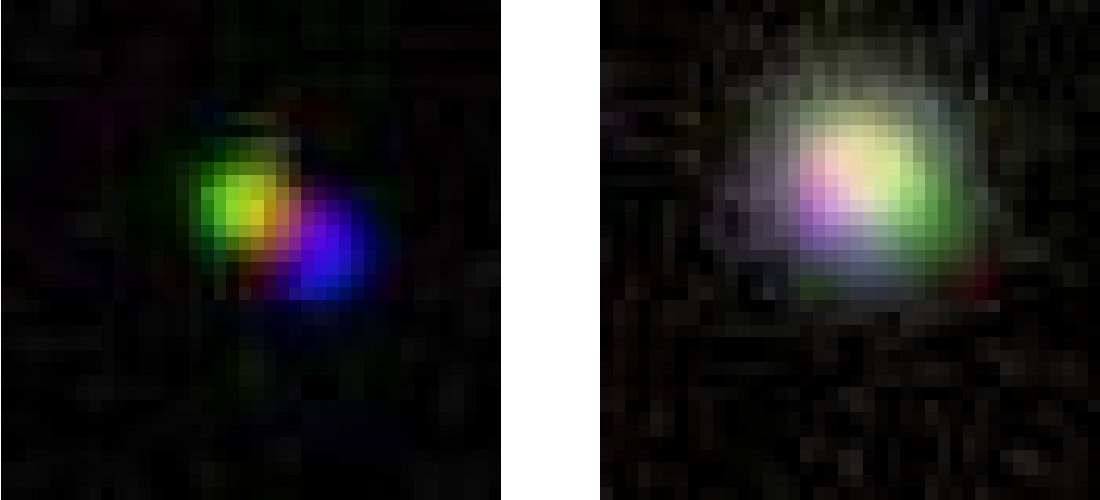
\includegraphics[width=80mm]{refs/pair.png}
\caption{An example of an asteroid in the Sloan Digital Sky Survey dataset
(left) and a non-asteroid body (right).}
\end{figure}

\section{Approach}
Here, we discuss the approach we took to classify the data using a neural
network.

\subsection{Initial training data}
First, we used a small tool to extract potential candidates from the full-scale
images which comprise the data set of the Sloan Digital Sky Survey. This tool
took an extremely na\"{\i}ve approach to selecting candidate asteroids,
producing nearly 100 false-positives for every 5 true positives it found.
Similarly, it acted conservatively with false-negatives, producing only
approximately one false-negative for every 1000 true negatives. This is also due
to the majority of artifacts being true negatives.

\begin{figure}
\centering
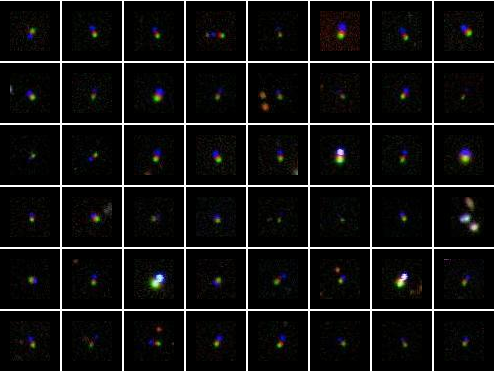
\includegraphics[width=80mm]{refs/valid.png}
\caption{Several individual verified asteroids.}
\end{figure}

This approach was good to build the training data set, but required manual
classification to verify the results, and the algorithm was extremely slow and
inefficient for any large-scale type of processing. As a result, it yielded
approximately 250 valid data points and 500 ``invalid'' or negative points.

\begin{figure}
\centering
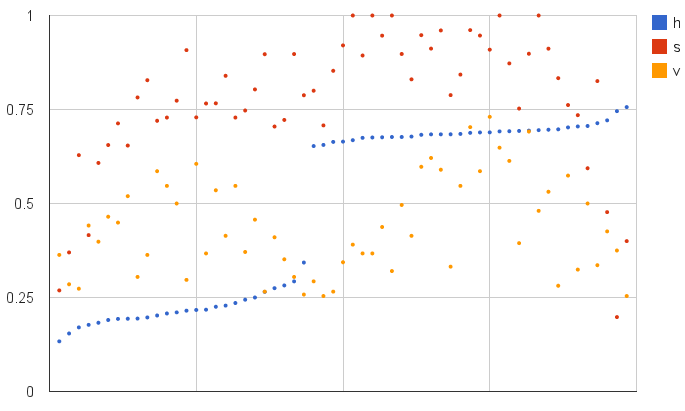
\includegraphics[width=80mm]{refs/chart_1.png}
\caption{Plotting an asteroid in HSV space, where $0.25 < v < 0.75$, reveals two
distinct hues.}
\end{figure}

\subsection{Feature: Valid Hue Ratio}
An important classifier for this subset of objects is matching the colors, also
known as the ``hues'' to hues which result from the ``shifting'' of the object
across various exposures. Each hue is representative of a different exposure
plate, and therefore has a relatively predictable value. 

Using the training data, we can predict what the ideal value for the two hues
which make up a valid asteroid, and use these to compare with other hues present
in the search space for the particular artifact. By filtering out high and low
values at each end of the spectrum, we ensure good results for our valid hue
ratio, which is not affected by over- or under-exposure.

Images with a majority of hues in the correct groupings will have hue ratio
values close to $1$, whereas images which are lacking high percentages of the
correct hue values will have a hue ratio close to $0$.

\subsection{Feature: Cluster Collinearity}
To compute this feature, as well as the third and final feature, it is necessary
to take the valid hue points from the previous feature and apply $k$-means
clustering to the point set, to determine a set of three clusters. In an ideal
image, these three clusters will correspond to each of the two plate exposures
for the moving body, as well as the intermediate hues which often lie between
these exposures.

This method produces three centroids for the hue points, which we can then use
for the second and third feature sets. For both features, we iterate the
$k$-means clustering a number of times, to produce an optimal clustering.

For cluster collinearity, we determine the degree to which the three center
points of these clustered centroids are collinear, that is, that they sit upon
the same line. An image with a low collinearity value is an image where the
exposure clusters move linearly, whereas an image with a high collinearity value
has no such linear component. Therefore, a perfectly collinear set of three
points will have a collinearity feature of $0$, and three points which have the
maximum possible collinearity have a collinearity feature of $1$.

\subsection{Feature: Mean Cluster Distance}
Similar to the clustered collinearity feature, the mean cluster distance feature
also uses the same $k$-means clustering of the first feature's hue values. Here,
we attempt to define a feature which represents how ``close-knit'' a given
cluster's points are to it's center, where a low value would represent a
relatively small average distance, and a high value (for a non-asteroid, for
example) would represent a relatively large average distance.

\begin{figure}
\centering
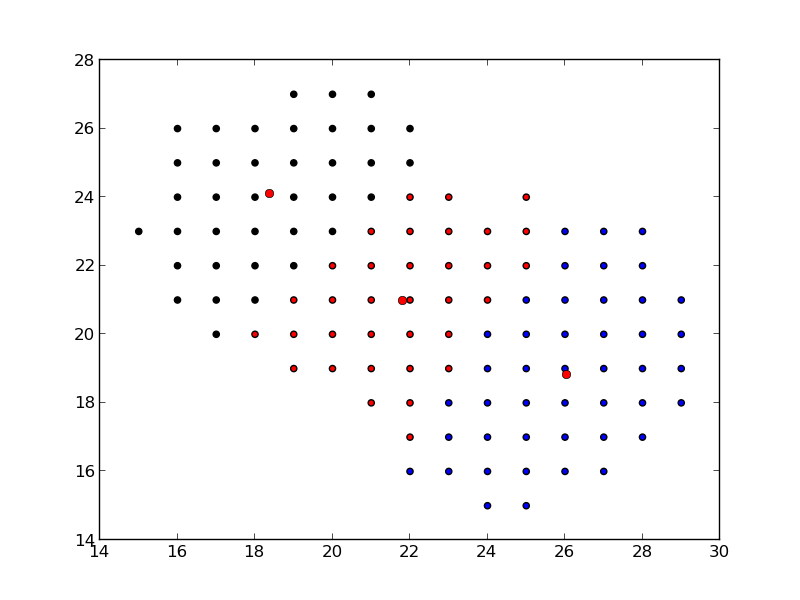
\includegraphics[width=80mm]{refs/clust-18364.png}
\caption{The result of $k$-means clustering of a valid asteroid, where $k=3$.}
\end{figure}

\begin{figure}
\centering
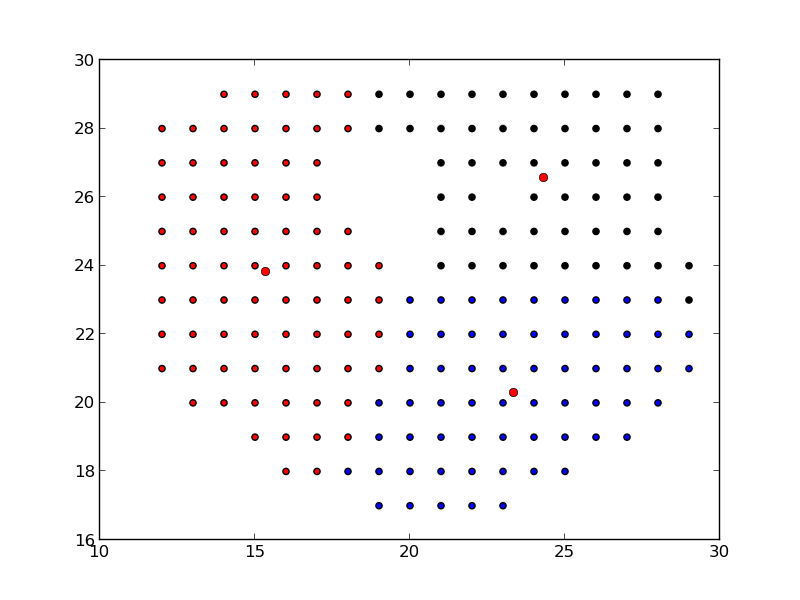
\includegraphics[width=80mm]{refs/clust-494.png}
\caption{The result of $k$-means clustering of a non-valid asteroid, where $k=3$.}
\end{figure}

\subsection{Building the Neural Network}
The resulting neural network uses supervised learning with the aforementioned
initial data set to build the trainer. We use Pybrain~\cite{pybrain} and use
backpropagation with three network layers: an input layer with three neurons,
corresponding to the three features we have defined in previous subsections, a
hidden layer with four hidden neurons, and a output layer with a single neuron,
which corresponds to the classification that the network gives to the input data
upon activation. This configuration, paired with a learning rate $r = 0.01$ and
momentum $p = 0.99$ (which was found to be optimal after a significant amount of
trial and error) produced good results when training the network.

\begin{figure}
\centering
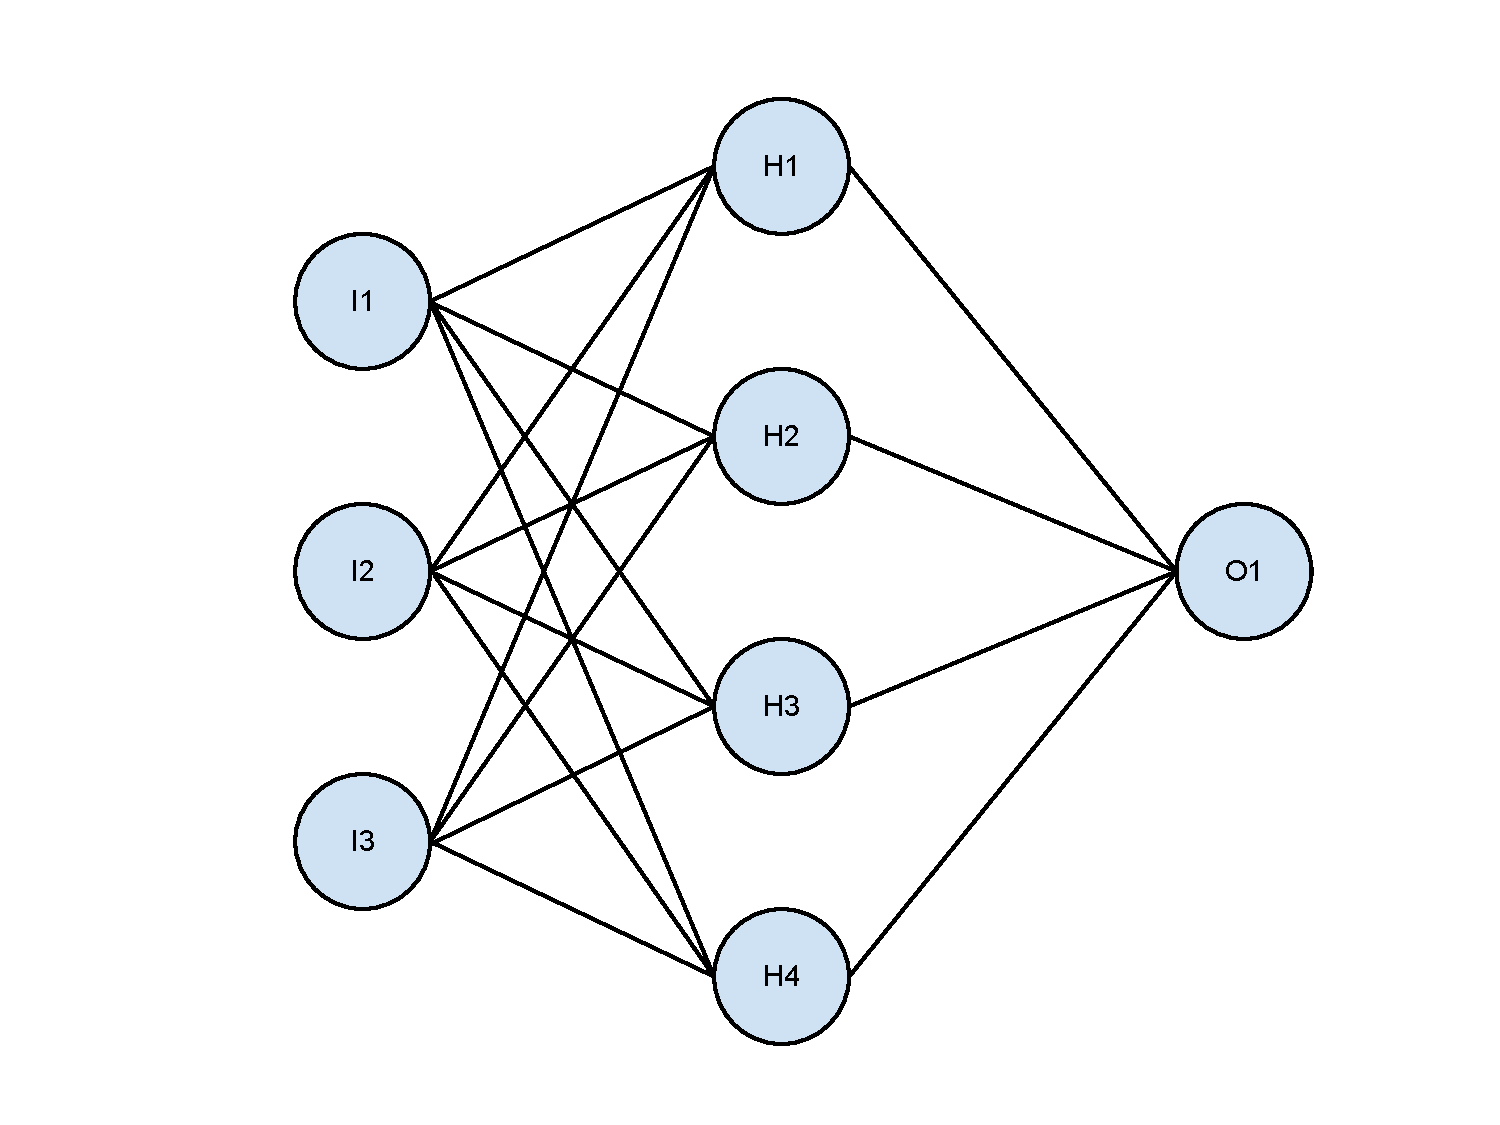
\includegraphics[width=90mm]{refs/nn.pdf}
\caption{The resulting neural network graph.}
\end{figure}

\subsection{Training the Neural Network}
Using the approximately 250 valid data points and 500 invalid data points, we
were able to train the neural network with the previously mentioned
configuration for five thousand iterations to reach a ``good enough''
convergence. The final training session took nearly three hours.

\section{Evaluation}
The best way to evaluate the quality of our neural network is to test it on a
series of data sets which were not included in the training data. We define
three individual and unique data sets, and outline the result the quality of
the results in the following figures.

    \begin{figure}
    \centering
    {\footnotesize
    \begin{tabular}{|c|c|c|c|c|c|c|c|}
        \hline
        \textbf{Trial} &  \textbf{Found Valid} & \textbf{Actual Valid} &
        \textbf{Total} & \textbf{False positive} \\\hline
        Trial 1 &   8 &   5 &   190 & 37.50\% \\\hline
        Trial 2 & 23 &  21 &  286 & 8.70\% \\\hline
        Trial 3 & 54 &  46 &  955 & 14.81\% \\\hline
    \end{tabular}
    }
    \caption{Results of valid images and false positives after three trials.}
    \end{figure}

    \begin{figure}
    \centering
    {\footnotesize
    \begin{tabular}{|c|c|c|c|c|c|c|c|}
        \hline
        \textbf{Trial} &  \textbf{Found Invalid} & \textbf{Actual Invalid} &
        \textbf{Total} & \textbf{False negative} \\\hline
        Trial 1 & 182 & 182 & 190 & 0.00\% \\\hline
        Trial 2 & 263 & 262 & 286 & 0.38\% \\\hline
        Trial 3 & 901 & 892 & 955 & 1.00\% \\\hline
    \end{tabular}
    }
    \caption{Results of invalid images and false negatives after three trials.}
    \end{figure}

\section{Conclusion}
To conclude, we find that a simple neural network with a well defined, yet
concise feature set produces a valid and accurate classifier. The majority of
the hard work is done in determining the feature set, and by the heavy lifting
done by the neural network itself. When paired with a human for validation of
false-positives and false-negatives, the process would become very quick and
very accurate at predicting the desired features.

\bibliographystyle{IEEEtran}
\bibliography{astro}
~\\
~\\
~\\
{ \footnotesize
\textbf{NOTE:} You might notice that this paper has nothing to do with my
originally proposed topic, ``Behavior Identification and Predictive Analysis of
Philadelphia Parking Authority Agents.'' After collecting and sanitizing a large
amount of data for the project, and beginning some initial analysis, it became
clear the there were two issue: first, that the data was still far too messy to
produce any meaningful output, and more importantly, that the ``AI problem''
which should be at the root of the project was becoming increasingly hard to
find. Therefore, I quickly changed gears, or ``pivoted,'' if you prefer, to this
problem, which proved to be much more interesting (and, possibly, useful) in the
end.
}

\end{document}
